\chapter{Reference Signals}

%---------- Overview ----------%
\section{Overview}
Reference signals are predefined signals occupying specific resource elements within the down-link time-frequency grid. The NR specification includes several types of reference signals transmitted in different ways and intended to be used for different purposes by a receiving device.
\newline
Unlike LTE, which relies heavily on always-on, cell-specific reference signals in the down-link for coherent demodulation, channel quality estimation for CSI reporting, and general time-frequency tracking, NR uses different down-link reference signals for different purposes. This allows for optimizing each of the reference signals for their specific purpose. It is also in line with the overall principle of ultra-lean transmission as the different reference signals can be transmitted only when needed. Later release of LTE took some steps in this direction, but NR can exploit this to a much larger degree as there are no legacy NR devices to cater for.
\newline
The NR reference signals include:
\begin{itemize}
    \item Demodulation reference signals (DMRS) for PDSCH are intended for channel estimation at the device as part of coherent demodulation. They are present only in the resource blocks used for PDSCH transmission. Similarly, the DMRS for PUSCH allows the gNB to coherently demodulate the PUSCH.
    \item Phase-tracking reference signals (PTRS) can be seen as an extension to DMRS for PDSCH/PUSCH and are intended for phase-noise compensation. The PT-RS is denser in time but sparser in frequency than the DM-RS, and, if configured, occurs only in combination with DMRS.
    \item CSI reference signals (CSI-RS) are downlink reference signals intended to be used by devices to acquire down-link channel-state information (CSI). Specific instances of CSI reference signals can be configured for time/frequency tracking and mobility measurements.
    \item Tracking reference signals (TRS) are sparse reference signals intended to assist the device in time and frequency tracking
    \item Sounding reference signals (SRS) are uplink reference signals transmitted by the devices and used for uplink channel-state estimation at the base stations.
\end{itemize}

The previous section assumed full knowledge of the channel characteristics at both transmitter and receiver sides, this section discusses how such knowledge is gained by focusing on two important reference signals : CSI-RS and DMRS.
\newline
The propagation channel depends on the transmit frequency. Therefore, if up-link and down-link operate on two different frequencies as is the case in FDD, there is no choice but relying on the receiver to communicate information about the channel back to the transmitter. This is the case at the bottom right.
\newline
In the case of TDD, where the up-link and down-link share the same transmit frequency, it is possible, on the other hand, to estimate the down-link channel based on measurements on up-link transmission (or the opposite). In this section we focus on the FDD transmission case.
%------------------------------%

%------------ DMRS ------------%
\section{Demodulation Reference signal (DMRS)}
The DM-RS in NR provides quite some flexibility to cater for different deployment scenarios and use cases: a front-loaded design to enable low latency, support for up to 12 orthogonal antenna ports for MIMO, transmissions duration from 2 to 14 symbols, and up to four reference-signal instances per slot to support very high-speed scenarios.
To achieve low latency, it is beneficial to locate the demodulation reference signals early in the transmission, sometimes known as front-loaded reference signals. This allows the receiver to obtain a channel estimate early and, once the channel estimate is obtained, process the received symbols on the fly without having to buffer a complete slot prior to data processing. This is essentially the same motivation as for the frequency-first mapping of data to the resource elements.
Two main time-domain structures are supported, differing in the location of the first DM-RS symbol:
\begin{itemize}
    \item Mapping type A, where the first DMRS is located in symbol 2 or 3 of the slot and the DMRS is mapped relative to the start of the slot boundary, regardless of where in the slot the actual data transmission starts. This mapping type is primarily intended for the case where the data occupy (most of) a slot. The reason for symbol 2 or 3 in the down-link is to locate the first DMRS occasion after a CORESET located at the beginning of a slot.
    \item Mapping type B, where the first DMRS is located in the first symbol of the data allocation, that is, the DMRS location is not given relative to the slot boundary but rather relative to where the data are located. This mapping is originally motivated by transmissions over a small fraction of the slot to support very low latency and other transmissions that benefit from not waiting until a slot boundary starts but can be used regardless of the transmission duration.
\end{itemize}

\begin{figure}[ht]
\centering
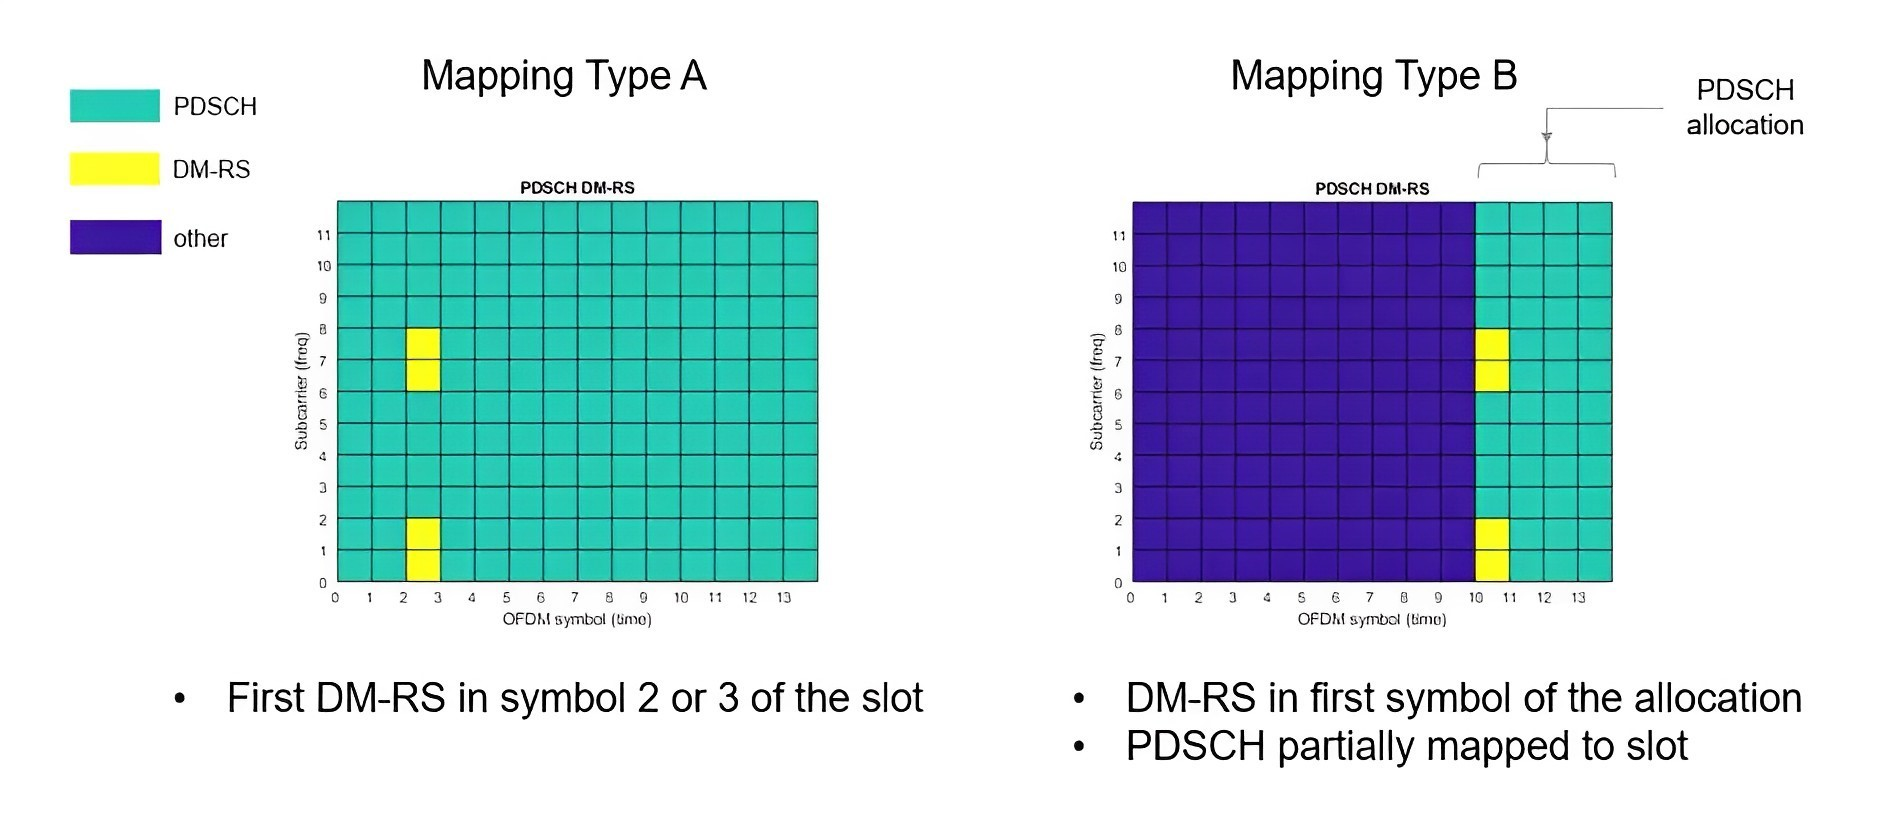
\includegraphics[width=0.6 \textwidth]{6-2.jpg}
\caption{DMRS Mapping type A \& type B }
%\label{fig:figure4.1}
\end{figure}

Although front-loaded reference signals are beneficial from a latency perspective, they may not be sufficiently dense in the time domain in the case of rapid channel variations. To support high-speed scenarios, it is possible to configure up to three additional DM-RS occasions in a slot. The channel estimator in the receiver can use these additional occasions for more accurate channel estimation, for example, to use interpolation between the occasions within a slot.

\subsection{Pilot based DMRS channel estimation}
\begin{wrapfigure}{r}{0.4\textwidth}
    \centering
    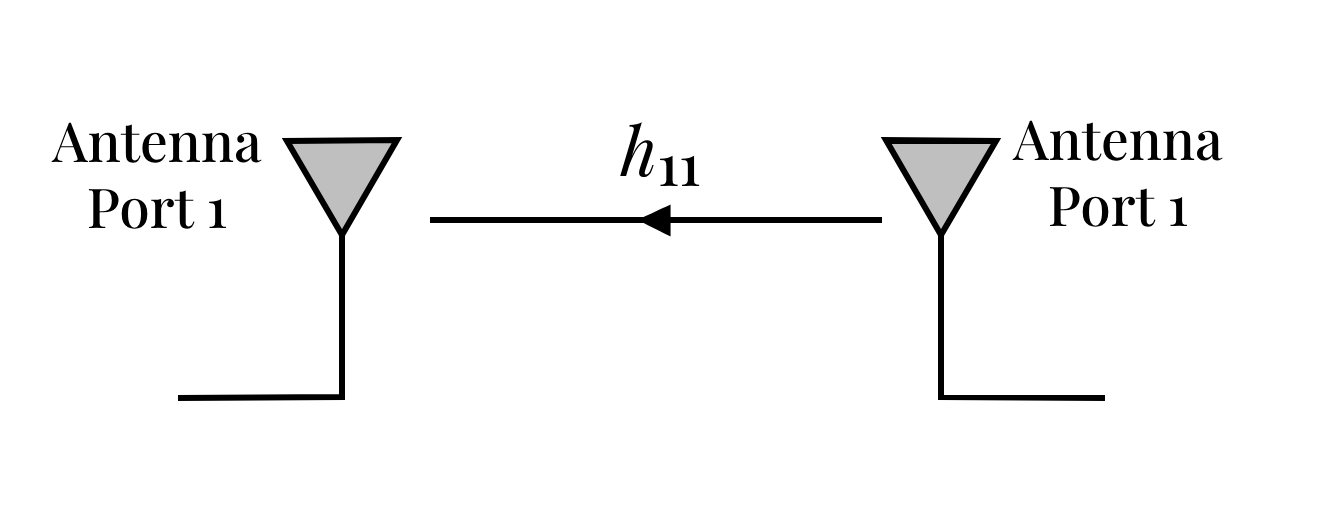
\includegraphics[width=0.4\textwidth]{7.png}
    \caption{Single Tx Single Rx}
    \label{fig:Single Tx Single Rx}
\end{wrapfigure}

Assume a single antenna port at both Tx and Rx.
\[ y = h_{11} x \]
In order to know $h_11$, we need to send a symbol $x$ which is known at the receiver, then $h_11$ can be calculated as:
\[ h_{11} = \frac{y}{x} \]

This known symbol $x$ is called a pilot symbol.
The problem with this approach is that there exists a channel coefficient need to be known for each RE in the PDSCH which requires sending pilots in all REs, hence there will not be any place for data bits.
The solution to this problem is to send pilot symbols in some REs as shown in the figure to determine the channel coefficients in those REs.

\begin{figure}[ht]
\centering
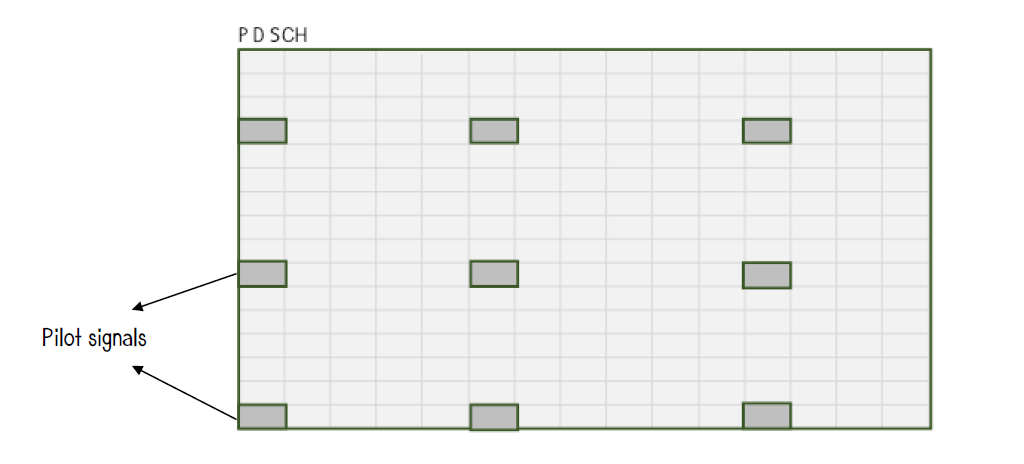
\includegraphics[width=6.47 in, height=2.36in]{8.PNG}
\caption{Pilot signals in some REs}
%\label{fig:figure4.1}
\end{figure}     

Use time/frequency correlation to determine channel coefficients in other REs

\begin{figure}[ht]
\centering
    \begin{subfigure}[b]{0.4\textwidth}
        \centering
        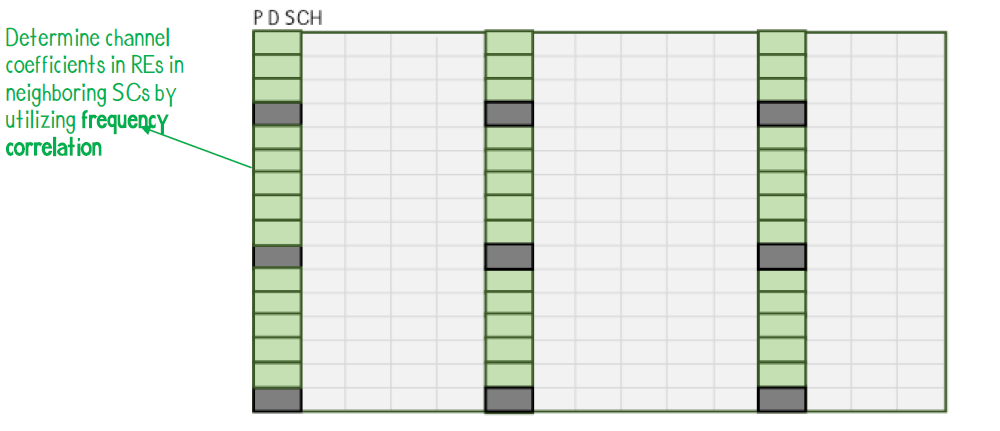
\includegraphics[width=\textwidth]{9.PNG}
        \caption{Frequency correlation }
    \end{subfigure}
    \hfill
    \begin{subfigure}[b]{0.4\textwidth}
        \centering
        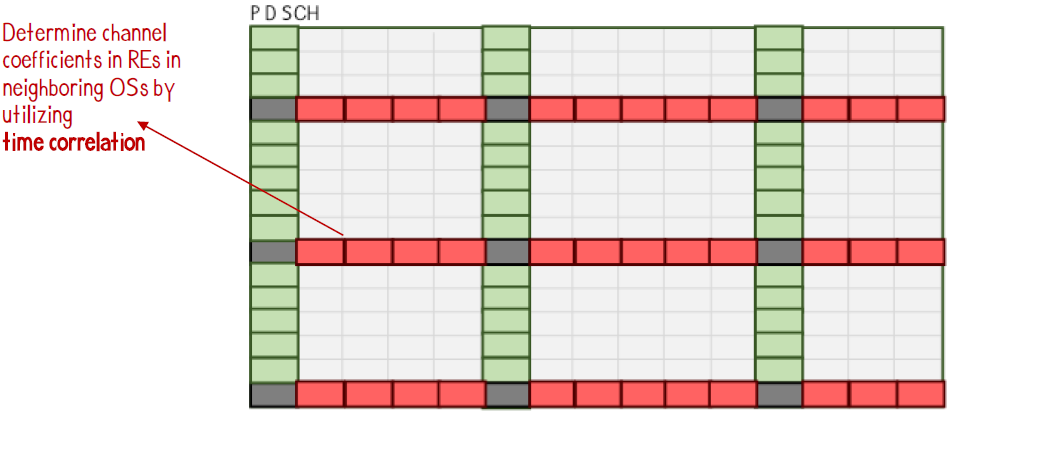
\includegraphics[width=\textwidth]{10.PNG}
        \caption{Time correlation }
    \end{subfigure}
    \hfill
    \begin{subfigure}[c]{0.4\textwidth}
        \centering
        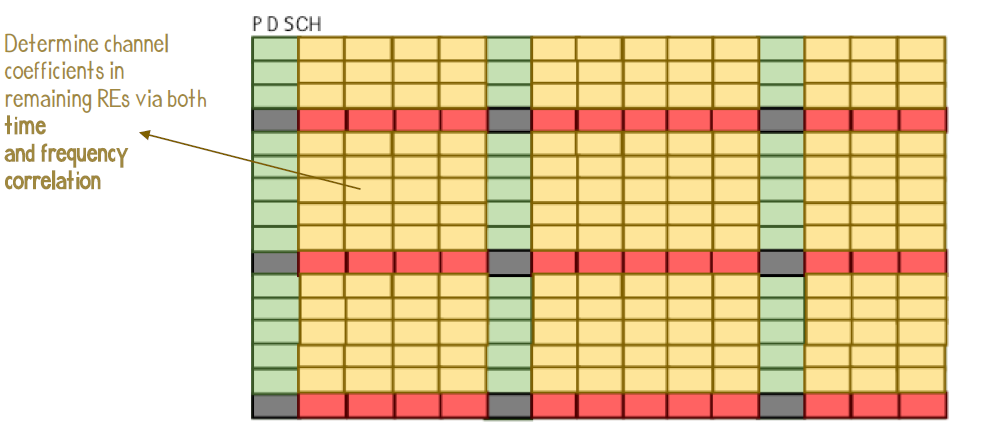
\includegraphics[width=\textwidth]{11.PNG}
        \caption{Time / frequency correlation }
    \end{subfigure}
       \caption{Correlation in time \& frequency}
\end{figure}

For the above property to be used time and frequency correlations must be determined, these are known using coherence time and coherence bandwidth.
\newline\newline
Coherence bandwidth is a statistical measurement of the range of frequencies over which the channel can be considered "flat", or in other words the approximate maximum bandwidth or frequency interval over which two frequencies of a signal are likely to experience comparable or correlated amplitude fading. If the multi-path time delay spread equals D seconds, then the coherence bandwidth $B_c$ is given approximately by the equation
\begin{equation}
    \label{Coherence bandwidth}
    B_c \approx \frac{1}{D}
\end{equation}

Hence if the delay spread is small, frequency correlation is high which means we need less pilots density in the frequency domain.
\begin{figure}[ht]
\centering
    \begin{subfigure}[b]{0.4\textwidth}
        \centering
        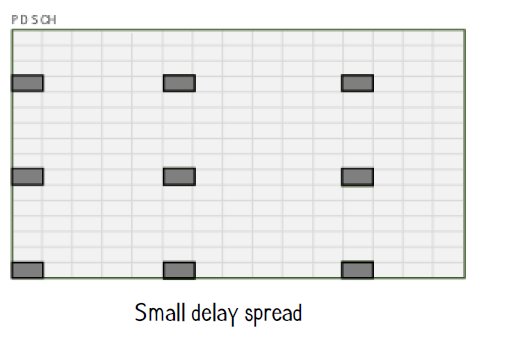
\includegraphics[width=\textwidth]{12.PNG}
        \caption{Small delay spread }
    \end{subfigure}
    \hfill
    \begin{subfigure}[b]{0.4\textwidth}
        \centering
        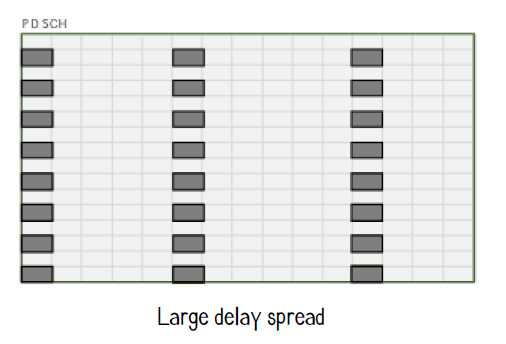
\includegraphics[width=\textwidth]{13.PNG}
        \caption{Large delay spread }
    \end{subfigure}
       \caption{Delay spread effect}
\end{figure}

Coherence time is the time duration over which the channel impulse response is considered to be not varying. Such channel variation is much more significant in wireless communications systems, due to Doppler effects. If the maximum doppler spread equals $f_m$ Hz, then the coherence time $T_c$ is given approximately by the equation
\begin{equation}
    \label{Coherence time}
    T_c \approx \frac{1}{f_m}
\end{equation}

Hence if the doppler spread is small, time correlation is high which means we need less pilots density in the time domain.

\begin{figure}[ht]
\centering
    \begin{subfigure}[b]{0.4\textwidth}
        \centering
        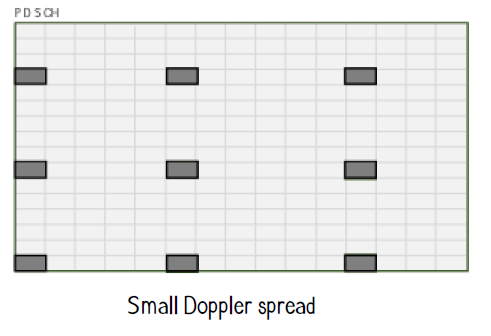
\includegraphics[width=\textwidth]{14.PNG}
        \caption{Small Doppler spread }
    \end{subfigure}
    \hfill
    \begin{subfigure}[b]{0.4\textwidth}
        \centering
        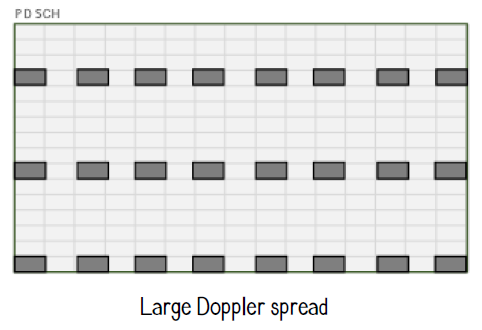
\includegraphics[width=\textwidth]{15.PNG}
        \caption{Large Doppler spread}
    \end{subfigure}
       \caption{Doppler spread effect}
\end{figure}
%-----------------------------%


%------------ CSI ------------%
\section{Channel State Information Reference Signal (CSI-RS)}
In the first release of LTE (release 8), channel knowledge for the downlink transmission direction was solely acquired by means of device measurements on the so-called cell-specific reference signals (CRS). The LTE CRS are transmitted over the entire carrier bandwidth within every LTE sub-frame of length 1 ms, and can be assumed to be transmitted over the entire cell area. Thus, a device accessing an LTE network can assume that CRS are always present and can be measured on.
\newline
In LTE release 10 the CRS were complemented by so-called CSI-RS. In contrast to CRS, the LTE CSI-RS are not necessarily transmitted continuously. Rather, an LTE device is explicitly configured to measure on a set of CSI-RS and does not make any assumptions regarding the presence of a CSI-RS unless it is explicitly configured for the device.
The origin for the introduction of CSI-RS was the extension of LTE to support spatial multiplexing with more than four layers, something which was not possible with the release-8 CRS. However, the use of CSI-RS was soon found to be an, in general, more flexible and efficient tool for channel sounding, compared to CRS. In later releases of LTE, the CSI-RS concept was further extended to also support, for example, interference estimation and multi-point transmission.
\newline
As already described, a key design principle for the development of NR has been to as much as possible avoid “always on” signals. For this reason, there are no CRS-like signals in NR. Rather, the only “always-on” NR signal is the so called SS block which is transmitted over a limited bandwidth and with a much larger periodicity compared to the LTE CRS. The SS block can be used for power measurements to estimate, for example, path loss and average channel quality. However, due to the limited bandwidth and low duty cycle, the SS block is not suitable for more detailed channel sounding aimed at tracking channel properties that vary rapidly in time and/or frequency.
\newline
Instead the concept of CSI-RS is reused in NR and further extended to, for example, provide support for beam management and mobility as a complement to SS block.
CSI-RS is a DL signal that can be used by the UE to measure some parameters and reports it back to the gNB to take actions based on that parameters.
Some of this parameters can be :
\begin{itemize}
    \item Channel quality indicator (CQI)
    \item Precoding matrix indicator (PMI)
    \item Rank indicator (RI)
\end{itemize}

\subsection{Basic CSI-RS structure}

A configured CSI-RS may correspond to up to 32 different antenna ports, each corresponding to a channel to be sounded. In NR, a CSI-RS is always configured on a per-device basis. It is important to understand though that configuration on a per-device basis does not necessarily mean that a transmitted CSI-RS can only be used by a single device. Nothing prevents identical CSI-RS using the same set of resource elements to be separately configured for multiple devices, in practice implying that a single CS-RS is shared between the devices.
\newline
As illustrated in Fig. 2.7, a single-port CSI-RS occupies a single resource element within a block corresponding to one resource block in the frequency domain and one slot in the time domain. In principle, the CSI-RS can be configured to occur anywhere within this block although in practice there are some restrictions to avoid collisions with other downlink physical channels and signals. Especially, a device can assume that transmission of a configured CSI-RS will not collide with:
\begin{itemize}
    \item Any CORESET configured for the device.
    \item Demodulation reference signals associated with PDSCH transmissions scheduled for the device. 
    \item Transmitted SS blocks.
\end{itemize}

\begin{figure}[h]
\centering
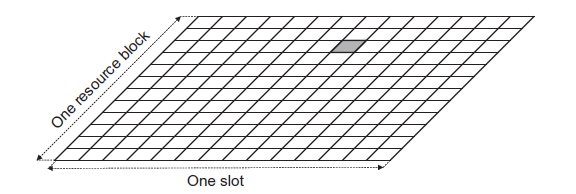
\includegraphics[width=4.8 in, height=1.62in]{16.PNG}
\caption{Single-port CSI-RS structure consisting of a single resource element within an RB/slot block. }
\end{figure}


\subsection{Frequency-Domain structure of CSI-RS configurations}

A CSI-RS is configured for a given downlink bandwidth part and is then assumed to be confined within that bandwidth part and use the numerology of the bandwidth part.
\newline
The CSI-RS can be configured to cover the full bandwidth of the bandwidth part or just a fraction of the bandwidth. In the latter case, the CSI-RS bandwidth and frequency-domain starting position are provided as part of the CSI-RS configuration. 
\newline
Within the configured CSI-RS bandwidth, a CSI-RS may be configured for transmission in every resource block, referred to as CSI-RS density equal to one.
\newline
However, a CSI-RS may also be configured for transmission only in every second resource block, referred to as CSI-RS density equal to 1/2. In the latter case, the CSI-RS configuration includes information about the set of resource blocks (odd resource blocks or even resource blocks) within which the CSI-RS will be transmitted. CSI-RS density equal to 1/2 is not supported for CSI-RS with 4, 8, and 12 antenna ports.
\newline
There is also a possibility to configure a single-port CSI-RS with a density of 3 in which case the CSI-RS occupies three subcarriers within each resource block. This CSI-RS structure is used as part of a so-called Tracking Reference signal (TRS).

\begin{figure}[h]
\centering
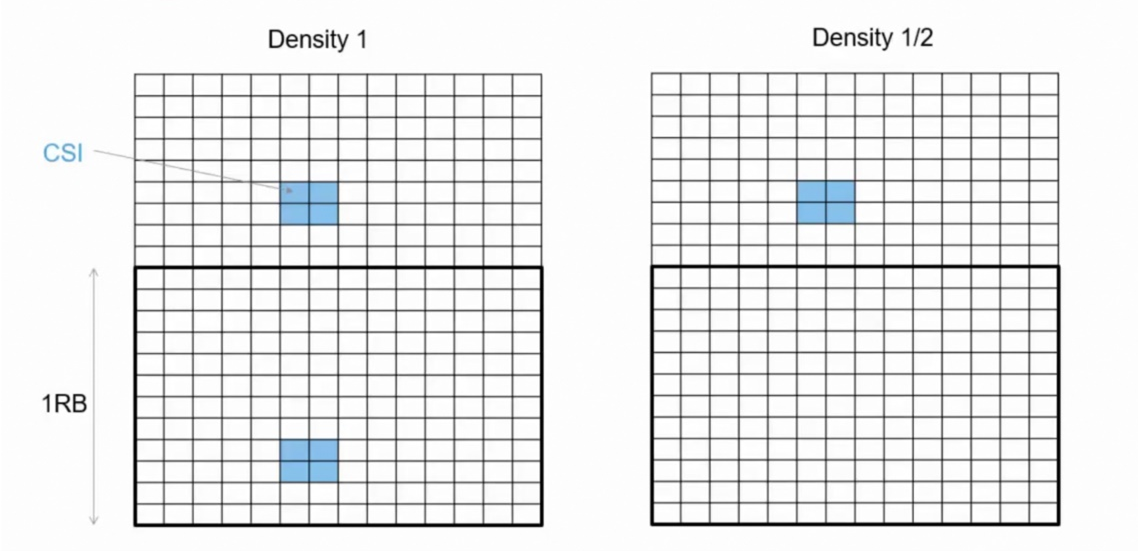
\includegraphics[width=5.17 in, height=2.51in]{17.PNG}
\caption{CSI-RS Frequency density }
\end{figure}

\subsection{Time-Domain structure of CSI-RS configurations}

The per-resource-block CSI-RS structure outlined above describes the structure of a CSI-RS transmission, assuming the CSI-RS is actually transmitted in a given slot. In general, a CSI-RS can be configured for periodic, semi-persistent, or aperiodic transmission.
\newline
In the case of periodic CSI-RS transmission, a device can assume that a configured CSI-RS transmission occurs every Nth slot, where N ranges from as low as four, that is, CSI-RS transmissions every fourth slot, to as high as 640, that is, CSI-RS transmission only every 640th slot. In addition to the periodicity, the device is also configured with a specific slot offset for the CSI-RS transmission
\newline
In the case of semi-persistent CSI-RS transmission, a certain CSI-RS periodicity and corresponding slot offset are configured in the same way as for periodic CSI-RS transmission. However, actual CSI-RS transmission can be activated/ deactivated based on MAC control elements (MAC CE). Once the CSI-RS transmission has been activated, the device can assume that the CSIRS transmission will continue according to the configured periodicity until it is explicitly deactivated. Similarly, once the CSI-RS transmission has been deactivated, the device can assume that there will be no CSI-RS transmissions according to the configuration until it is explicitly re-activated.
\newline
In the case of aperiodic CSI-RS, no periodicity is configured. Rather, a device is explicitly informed (“triggered”) about each CSI-RS transmission instant by means of signaling in the DCI.


\begin{figure}[h]
\centering
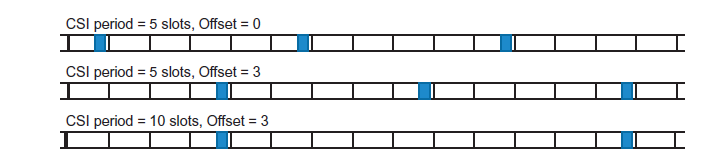
\includegraphics[width=6.47 in, height=1.45in]{18.PNG}
\caption{CSI-RS Periodicity and slot offset }
\end{figure}

\subsection{CSI-RS and DMRS for full channel estimation}
DMRS is used to help the receiver determine the effective channel, i.e., after taking into account the effect of the precoding matrix.
\newline
The question is how to determine the best precoding matrix ? CSI-RS is the answer.
Channel estimation process steps are as follows:
\begin{itemize}
    \item CSI-RS is transmitted to the UE to make initial channel estimation.
    \item A CSI feedback is sent to the gNB to be used to choose the necessary precoding, keep in mind that it is not necessary that the gNB uses the precoding suggested by the UE.
    \item PDSCH and its DMRS are transmitted after applying the chosen precoding.
    \item DMRS is used by the UE to estimate the effective channel after taking into account the effect of the precoding.
\end{itemize}


\begin{figure}[h]
\centering
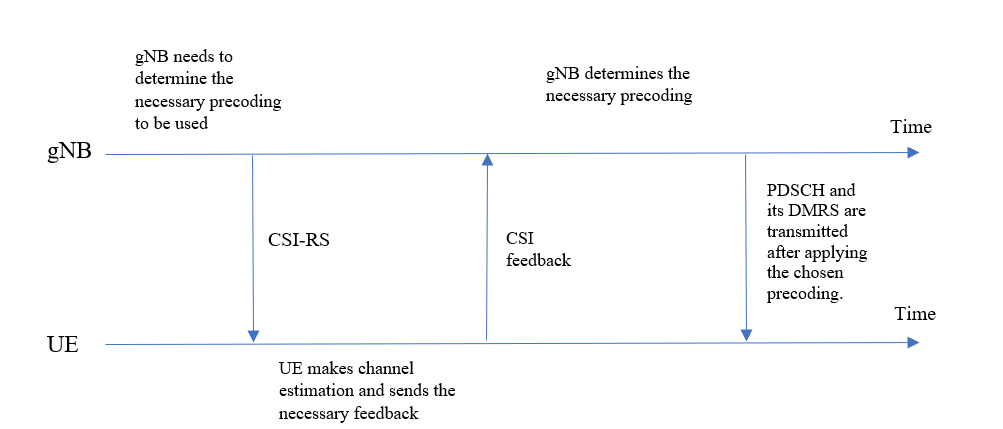
\includegraphics[width=6.07 in, height=2.6in]{19.PNG}
\caption{Channel estimation process }
\end{figure}
%-----------------------------%

%---- Channel Estimation -----%
\section{Channel Estimation}
In general, there are two types of MIMO channel estimation methods:
\begin{description}
    \item[Training based approach:] which uses known training symbols.
    \item[Blind-based approach:] which perform CE without the benefit of known training symbols.
\end{description}
In training-based CE, known training symbols are transmitted at certain prescribed times and frequencies that are known by the receiver. Since the receiver knows the training symbols, as well as when and where (i.e., at which frequencies) they are transmitted, it uses that information to estimate the gain and phase rotation imparted by the channel at each point in time and frequency based on the characteristics of the received training symbols. Although blind-based methods have higher bandwidth efficiencies because they do not use any resources for transmitting training symbols, they tend to have lower speed and poorer performance than training-based methods. For this reason, training-based CE is used more than blind-estimation, and it is the method we focus on in our project.

The placement of training symbols in time, frequency, and space (i.e., the transmit antenna’s) dimensions is a key part of the design of a MIMO communication system.
In general, training symbols should be spaced as far apart as possible to reduce training overhead, while still maintaining a required performance level. For example, in a high Doppler, fast fading environment, training symbols need to be placed relatively often in time. Similarly, in a highly frequency-selective channel, training symbols need to be placed close together in the frequency dimension.
In this section we discuss two channel estimation methods :
\begin{itemize}
    \item Simple pilot based estimation
    \item MMSE estimation
\end{itemize}

\subsection{Simple pilot based estimation}
\label{subsection:SPBE}

\begin{wrapfigure}{r}{0.4\textwidth}
    \centering
    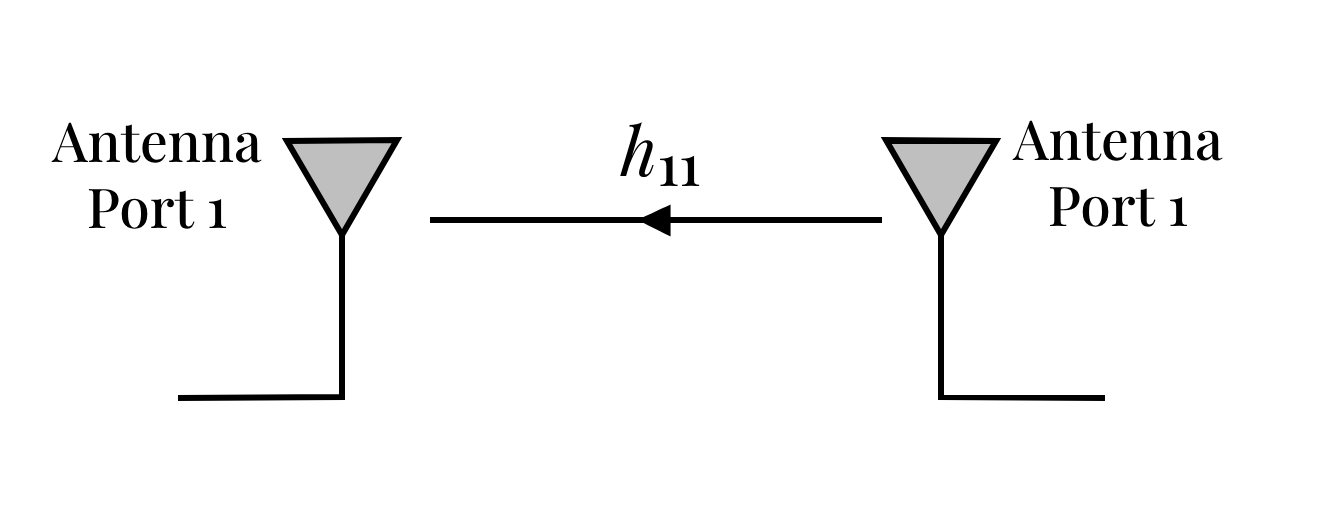
\includegraphics[width=0.4\textwidth]{7.png}
    \caption{Single Tx Single Rx}
\end{wrapfigure}
Assume a single antenna port at both Tx and Rx
\[ y = h_{11}x  \]

In order to know $h_{11}$, we need to send  a symbol x 
Which is known at the Rx, then $h_{11}$ can be known as                  
\[h_{11} = \frac{y}{x}\]
This known symbol $x$ is called a \emph{pilot symbol.}

\begin{wrapfigure}{r}{0.4\textwidth}
    \centering
    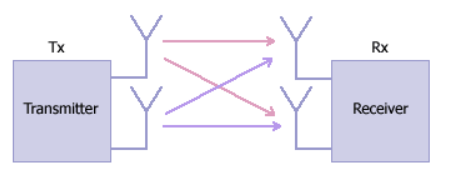
\includegraphics[width=0.4\textwidth]{20.PNG}
    \caption{2x2 MIMO setup}
    \label{fig:2x2MIMO}
\end{wrapfigure}

\textbf{What about a MIMO channel ?} \\
Assume a 2x2 MIMO setup as shown in Figure~\ref{fig:2x2MIMO}
\newline
The received signal y at the receiver side is 
\[y =\begin{bmatrix} y_1 \\ y_2 \end{bmatrix} = \begin{bmatrix} h_{11} & h_{21}  \\ h_{12} & h_{22} \end{bmatrix} \times \begin{bmatrix} x_1 \\ x_2 \end{bmatrix}  \]

Estimating the 4 channel coefficients is not as simple as the SISO case, to do so one pilot symbol won't be enough, a number of pilot symbols equal the number of transmit antennas will be needed.

\begin{figure}[ht]
\centering
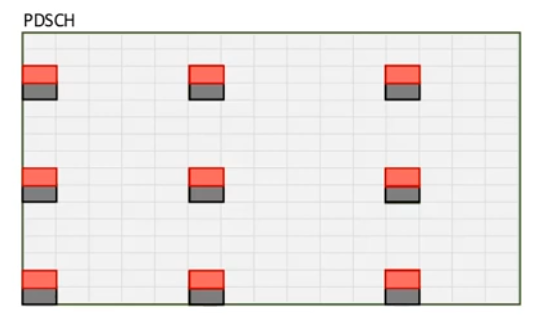
\includegraphics[width=0.4\textwidth]{21.PNG}
\caption{pilot symbols for 2x2 MIMO channel}
\end{figure} 

On the grey REs, pilots from the first layer only are sent

\[y =\begin{bmatrix} y_1 \\ y_2 \end{bmatrix} = \begin{bmatrix} h_{11} & h_{21}  \\ h_{12} & h_{22} \end{bmatrix} \times \begin{bmatrix} p_1 \\ 0 \end{bmatrix} =  \begin{bmatrix} h_{11} \\ h_{12}  \end{bmatrix}p_1\]

Knowing the value of the pilot symbol at the receiver side the channel coefficients corresponding to the first Tx layer can be estimated.
\newline
The same is done on the red REs with pilots from the second layer only are send, hence, the channel coefficients corresponding to the second Tx layer can be estimated.
\newline
This means that a number of pilot symbols equals the number of Tx layers is needed to fully estimate a MIMO channel. \\

The problem with this estimation method is that in the presence of noise the estimated channel coefficients are not exactly the real coefficients which results in errors in both precoding and decoding operations at the Tx and Rx. This problem appears clearly specially when estimation is done for two reference signals (i.e., CSI-RS and DMRS) where CSI-RS is used to choose the necessary precoding then DMRS is used to estimate the effective channel at the receiver side for decoding operation, the accumulated error in both estimations becomes big which results in a poor BER performance.

\subsection{Minimum mean square error (MMSE) estimation}

In MMSE the same approach as simple pilot based estimation (as mentioned in subsection~\ref{subsection:SPBE}) is done but the difference is that MMSE estimation takes into account the noise effect to get a better estimate of the channel coefficients. \\
For the channel model $y=Hx+n$ the channel estimate \^{H} is given as
\begin{equation}
    \displaystyle
    \label{Estimated channel using MMSE}
    \hat{H} = R_{hy} R_{yy} (\bar{y} - \bar{\mu_y}) + \mu_n
\end{equation}
\[ \text{where} \quad R_{hy} = \mathbb{E}\{ (h - \mu_h) (\bar{y} - \bar{\mu_y})^T \} \quad \text{is the cross covariance of } H, y\]
\[ \text{and} \quad R_{yy} = \mathbb{E}\{ (\bar{y} - \bar{\mu_y}) (\bar{y} - \bar{\mu_y})^T \} \quad \text{is the covariance matrix of } y\]
\[ \bar{\mu_y} \quad , \quad \mu_n \quad \text{are the expected value of } y \text{ and } n \text{ respectively.} \]

Using some mathematical manipulation we get that the estimate value of the channel can be given by this simplified expression
\begin{equation}
    \label{Estimated channel using MMSE (simplified equation)}
    \hat{H} = \frac{ \frac{ \bar{x}^H \bar{y} }{N_o} + \frac{\mu_h}{\sigma^2_h}  }{ \frac{\|\bar{x}\|^2}{N_o} + \frac{1}{\sigma^2_h} }
\end{equation}
Although MMSE estimation is more computationally complex than simple pilot estimations it gives a better estimate of the channel coefficients and hence a better BER performance.

%-----------------------------%